\documentclass[xcolor=dvipsnames]{beamer}
\hypersetup{unicode}

\usepackage{adjustbox}
\usepackage[utf8]{inputenc}
\usepackage[croatian]{babel}
\usepackage{csquotes}
\MakeOuterQuote{"}
\usepackage{tikz}
\usetheme{Boadilla}
\usecolortheme{lily}

\definecolor{Coral}{RGB}{255, 111, 97}
\definecolor{DarkBluishGray}{RGB}{47,52,53}
\setbeamercolor{title}{fg=Coral, bg=white}
\setbeamercolor{frametitle}{fg=DarkBluishGray, bg=Coral}
\setbeamercolor{title in head/foot}{fg=Coral, bg=DarkBluishGray}
\setbeamercolor{author in head/foot}{fg=Coral, bg=DarkBluishGray}
\setbeamercolor{date in head/foot}{fg=Coral, bg=DarkBluishGray}
\setbeamercolor{block title}{bg=Coral,fg=DarkBluishGray}

\title{Posljednja zadaća}
\subtitle{Prezentacija u \emph{Beamer}u}
\author{\texorpdfstring{Katarina Šupe}{Katarina Supe}}
\institute[PMF--MO]{Prirodoslovno-matematički fakultet --- Matematički odsjek}
\date{\today}

\begin{document}
\begin{frame}[plain]
\titlepage
\end{frame}
\begin{frame}
\frametitle{Matematički softver}
\begin{columns}[t]
\column{.3\textwidth}
\begin{block}{\centering\emph{Jupyter Notebook (Python)}}
\centering
Koristili smo \emph{Jupyter Notebook} za interaktivno programiranje u \emph{Python}u.
\end{block}
\column{.3\textwidth}
\begin{block}{\centering\LaTeX}
\centering
Naučili smo koliko je \LaTeX{} koristan u matematičkom svijetu. 
\end{block}
\end{columns}
\end{frame}

\begin{frame}{Zadaće}
\begin{adjustbox}{width=\textwidth}
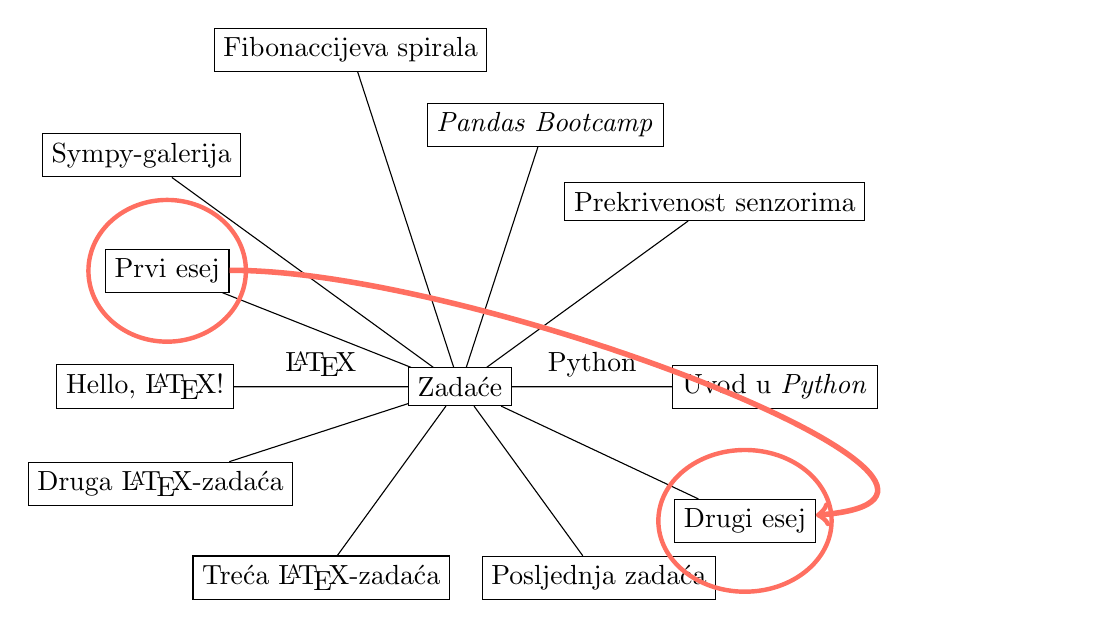
\begin{tikzpicture}
\tikzstyle{every node}=[draw,shape=rectangle];
\node (v0) at (0:0) {Zadaće};
\node (v1) at (0:4) {Uvod u \emph{Python}};
\node (v2) at (36:4) {Prekrivenost senzorima};
\node (v3) at (2*36:3.5) {\emph{Pandas Bootcamp}};
\node (v4) at (3*36:4.5) {Fibonaccijeva spirala};
\node (v5) at (4*36:5) {Sympy-galerija};
\node (esej1) at (4.4*36:4) {Prvi esej};
\node (v6) at (5*36:4) {Hello, \LaTeX!};
\node (v7) at (5.5*36:4) {Druga \LaTeX-zadaća};
\node (v8) at (6.5*36:3) {Treća \LaTeX-zadaća};
\node (v9) at (8.5*36:3) {Posljednja zadaća};
\node (esej2) at (9.3*36:4) {Drugi esej};
\draw (v0) -- (v1)
      (v0) -- (v2)
      (v0) -- (v3)
      (v0) -- (v4)
      (v0) -- (v5)
      (v0) -- (esej1)
      (v0) -- (v6)
      (v0) -- (v7)
      (v0) -- (v8)
      (v0) -- (v9)
      (v0) -- (esej2);
\path[every node/.style={sloped,anchor=south,auto=false}]
(v0) edge              node {Python} (v1)
(v0) edge              node {\LaTeX} (v6);
\pause
\draw[color=Coral, ultra thick] (esej1) ellipse (1 and 0.9);
\pause
\draw[color=Coral, ultra thick] (esej2) ellipse (1.1 and 0.9);
\pause
\draw[line width=2pt, color=Coral, ->] 
(esej1) 
to [out=0.5, in=4.7]
(esej2);
\end{tikzpicture}
\end{adjustbox}
\end{frame}
\begin{frame}{TikZ}
\begin{center}
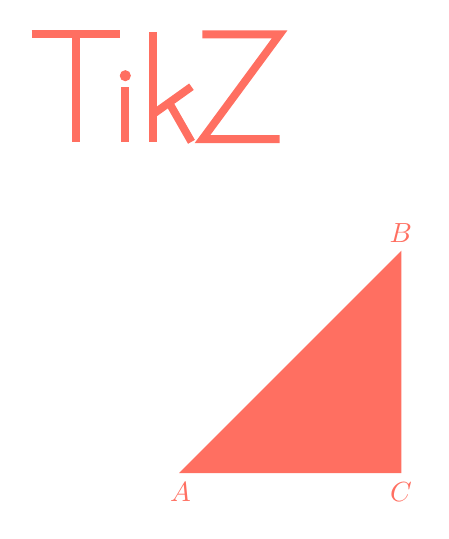
\begin{tikzpicture}[scale=0.7]
%\draw[help lines] (0,0) grid (15,10);
\draw[line width=1mm,Coral] (1.1,6) -- (1.1,8);
\draw[line width=1mm,Coral] (0.3,7.95) -- (1.9,7.95);
\draw[line width=1mm,Coral] (2,6) -- (2,7);
\draw[fill, Coral] (2,7.2) circle [radius=0.09];
\draw[line width=1mm,Coral] (2.5,6) -- (2.5,8);
\draw[line width=1mm,Coral] (2.5,6.5) -- (3.2,7);
\draw[line width=1mm,Coral] (2.8,6.7) -- (3.2,6);
\draw[line width=1mm,Coral] (3.4,7.95) -- (4.8, 7.95) -- (3.4, 6.05) -- (4.8, 6.05);
\draw[fill,Coral] (3,0) node[anchor=north]{$A$}
  -- (7,0) node[anchor=north]{$C$}
  -- (7,4) node[anchor=south]{$B$}
  -- cycle;
\end{tikzpicture}
\end{center}
\end{frame}
\begin{frame}{\emph{To-do list}}
Napiši \textbf<2>{sve} zadaće.

\only<3>{Napiši sve eseje.}
\end{frame}
\end{document}
